\documentclass[11pt]{article}
\usepackage{parskip} % Kerstin loves Luca!
\usepackage[USenglish]{babel}
\usepackage[T1]{fontenc} % Use 8-bit encoding that has 256 glyphs
\usepackage{geometry} % Document margins
\usepackage[toc,page]{appendix}
\usepackage{graphicx}
\usepackage{float} % allow for [H]
\usepackage[colorlinks=false,citecolor=black,linkcolor=black,bookmarks=true,bookmarksopen=false,bookmarksopenlevel=1,pagebackref, breaklinks=true, pdfborder={0 0 0}]{hyperref} % no boxes around hyperlinks in the PDF
\usepackage{url}
\usepackage{subcaption}
\usepackage{inconsolata} % font for code

% ================================================================
\title{Speed-up Using GPU Accelerators:  \\ 
How to Port a Numerical Solver for CFD with PyCUDA \\
\vspace*{0.75cm}\large Project for the PDC Summer School 2017}

\author{Kerstin Cramer \& Luca Manzari}
\date{February 2018}
% ================================================================
% ================================================================
\begin{document}
% ----------------------------------------------------------------
\maketitle
\tableofcontents
\newpage
% ----------------------------------------------------------------
\section{import Introduction}

In Computational Fluid Dynamics (CFD) non-linear conservation equations are solved for physical problems which are therefore discretized in space and time to allow local linearization of the equations. For each point of the grid and solving variable, a linear equation is obtained which needs to be solved for every time step. This results in a large system of linear equations growing with the refinement of the grid and the size of the physical problem. These characteristics qualify CFD codes for parallelization: they are commonly executed on Central Processing Units (CPUs) of high performance computers. 

Numerous linear equations are solved significantly faster with numerical, iterative methods. Using these methods, the problem is reduced to multiple matrix multiplications with big matrices. This single-instruction-multiple-data paradigm well fits the architecture of Graphical Processing Units (GPUs).

In this report, the process of porting a solver for non-symmetric linear systems of equations to run on GPUs is documented. The chosen solver is the bi-conjugate gradient stabilized (bicgstab) method which ranks as one of the fastest state-of-the-art numerical solvers for linear equations after multigrid methods. It is embedded into a laminar Navier-Stokes CFD code called pyns which is implemented in Python. Therefore, the PyCUDA module is used to translate Python code into NVIDIA CUDA kernels to achieve a speed-up of the overall execution time of the pyns code.

\section{import pyns.bicgstab as Problem}

The Finite-Volume code solves the incompressible Navier-Stokes equation in three dimensions. Following the SIMPLE algorithm, the momentum conservation equation is solved to obtain a preliminary velocity field. To ensure the conservation of mass, the pressure gradient is calculated from the pressure correction equation and is used to correct the velocity field. 

Both momentum conservation and pressure correction equations are discretized forming a system of linear equations. For each equation, seven system matrices are formed (one central and six for the neighboring directions). For their solution, an analytical solver, Krylov subspace methods and a multigrid solver are implemented. The implementation of the bicgstab method and the two subroutines it uses are discussed in this report.

\texttt{bicgstab} takes as input the seven system matrices, the matrix of the respective solving variable and the right-hand-side matrix of the linear equation to solve. Additionally, the desired tolerance and the maximum number of iterations can be set. In accordance with the bicgstab algorithm, new values for the solving variable are computed for the next time step in an iterative way using scalar operations and subroutines for matrix multiplication. 

\texttt{vec\_vec} calculates the vector-dot product of two matrices by performing an element-wise multiplication followed by a sum reduction.

\texttt{mat\_vec\_bnd} takes as input the seven system matrices and the matrix of the solving variable with its boundary values. The returned matrix represents the product of the left-hand side of the system of linear equations (the coefficient matrix multiplied with the solving variable). It does so by multiplying the central system matrix with the variable matrix and subtracting from it the results from the multiplication of the six neighbouring matrices with the solving variable matrix concatenated with the respective boundary values.

These three functions are ported and run on the GPU.

\section{import PyCUDA as Tool}

The PyCUDA module enables the execution of Python code on NVIDIA GPUs. Firstly, the \texttt{pycuda.driver} library has to be imported as it contains the CUDA functions. Secondly, the import of \texttt{pycuda.autoinit} is useful as it initializes automatically a context for evoking CUDA kernels. It probes for installed devices and decides on the number of blocks-per-grid and threads-per-block. Therefore, these parameters do not need to be modified or specified anymore. The context can also be set manually. 

The \texttt{pycuda.gpuarray} library offers convenient built-ins for handling numpy-compatible data types. Slicing of gpuarrays on the GPU is thereby supported and mathematical operations for gpuarrays are either built-in routines (like the matrix dot product) or offered in the \texttt{pycuda.cumath} library (like the sine function). Broadcasting and comparison operations are not clearly defined in PyCUDA. Multiplying a vector and a scalar both living on the GPU will multiply only the first element of the vector with the scalar. To correctly multiply a scalar and a vector that are on the GPU, the scalar needs to be fetched on the host: the multiplication is then carried out correctly on the GPU. The method \texttt{gpuarray.to\_gpu()} allocates memory and copies data from a numpy array to the GPU. To copy data into an existing gpuarray instance, the method \texttt{gpuarray.set()} can be used. Fetching data is performed calling the \texttt{gpuarray.get()} method. 

Other options that PyCUDA offers require some C code to be written. \texttt{ElementwiseKernel} from \texttt{pycuda.elementwise} takes an array as input, and runs the kernel on each element of the array. \texttt{ReductionKernel} from \texttt{pycuda.reduction} lets the user specify an elementwise operation (as in \texttt{ElementwiseKernel}) and a reduction operation to be executed afterwards. \texttt{SourceModule} from \texttt{pycuda.compiler} is a Python wrapper for native CUDA code.

\section{import Benchmarks as Approach}

The computations are run on the ULHPC Cluster Gaia on Intel Xeon E5-2680v3 CPUs and NVIDIA Tesla K80 GPUs when referred to Gaia. When referred to Tegner, the computations are carried out on KTH PDC Cluster Tegner on Intel E5-2690v3 Haswell CPUs and NVIDIA Tesla K80 GPUs. The code for the benchmarks can be found on github\footnote{\url{https://github.com/kjcramer/pyns/tree/HPC_SummerSchool/pycuda/benchmarks}}.

\subsection{Matrix Multiplication on CPU vs. \texttt{gpuarray}}

In this benchmark study, the elapsed time is compared when executing on the CPU versus on the GPU using \texttt{pycuda.gpuarray}. The matrix multiplication of two random, three dimensional matrices was performed 32, 64 and 128 times. The order of the matrices was varied between 64 and 256 in 16-increments.
Two different cases for copying the matrices to the GPU are thereby tested: whereas using \texttt{gpuarray.to\_gpu()}, memory for both matrices is allocated in each iteration anew followed by the copying of the values, using \texttt{gpuarray.set()}, it is only needed to copy the matrices' values each iteration into memory space which was preallocated in advance.

\begin{figure}[H]
    \centering
    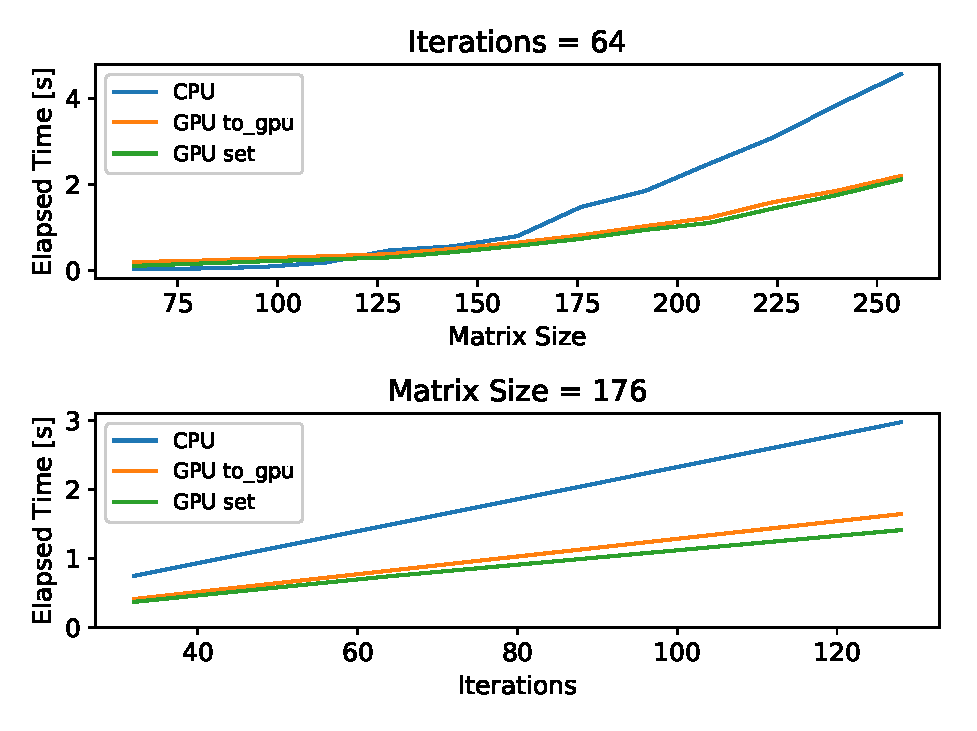
\includegraphics[width=0.7\textwidth]{benchmark001_outData_tegner_K80}
    \caption{Comparison of the run time of CPU and \texttt{gpuarray} methods: Elapsed time for matrix multiplication of three-dimensional matrices of order \emph{Matrix Size} after 64 iterations and influence of number of iterations on the elapsed time}
    \label{benchmark_002}
\end{figure}

The results shown in Figure~\ref{benchmark_002} are run on Tegner. The break-even-point between CPU and GPU execution time lies between the matrix order of 112 and 128. Also, \texttt{gpuarray.set()} is consistently faster than \texttt{gpuarray.to\_gpu()}, if an array needs to be written more than once, since the cost of the initialization and allocation is spared. The allocation time is independent of the amount of data that needs to be written.

\subsection{Sine Function on CPU vs. \texttt{gpuarray} vs. C Kernel vs. \texttt{Elementwise} Kernel}

This benchmark is taken from the PyCUDA example gallery\footnote{\url{https://wiki.tiker.net/PyCuda/Examples/SimpleSpeedTest}} and modified to include memory copying to the GPU in the time counting. It compares the execution time of the CPU and four methods to run on the GPU. The sine is computed of a one-dimensional vector with lengths between 16 to 256 with 16-increments for 100, 1000 and 10000 times. Using the \texttt{gpuarray} method, in every iteration the vector is send to the GPU where the sine is calculated using the \texttt{cumath} library (looping on the CPU). Two \texttt{Elementwise} kernels are compared: one of them loops on the GPU (\emph{EW w. loop}) whereas the other kernel is called in a loop on the CPU (\emph{EW}). Moreover, a C kernel is executed.

\begin{figure}[H]
    \centering
    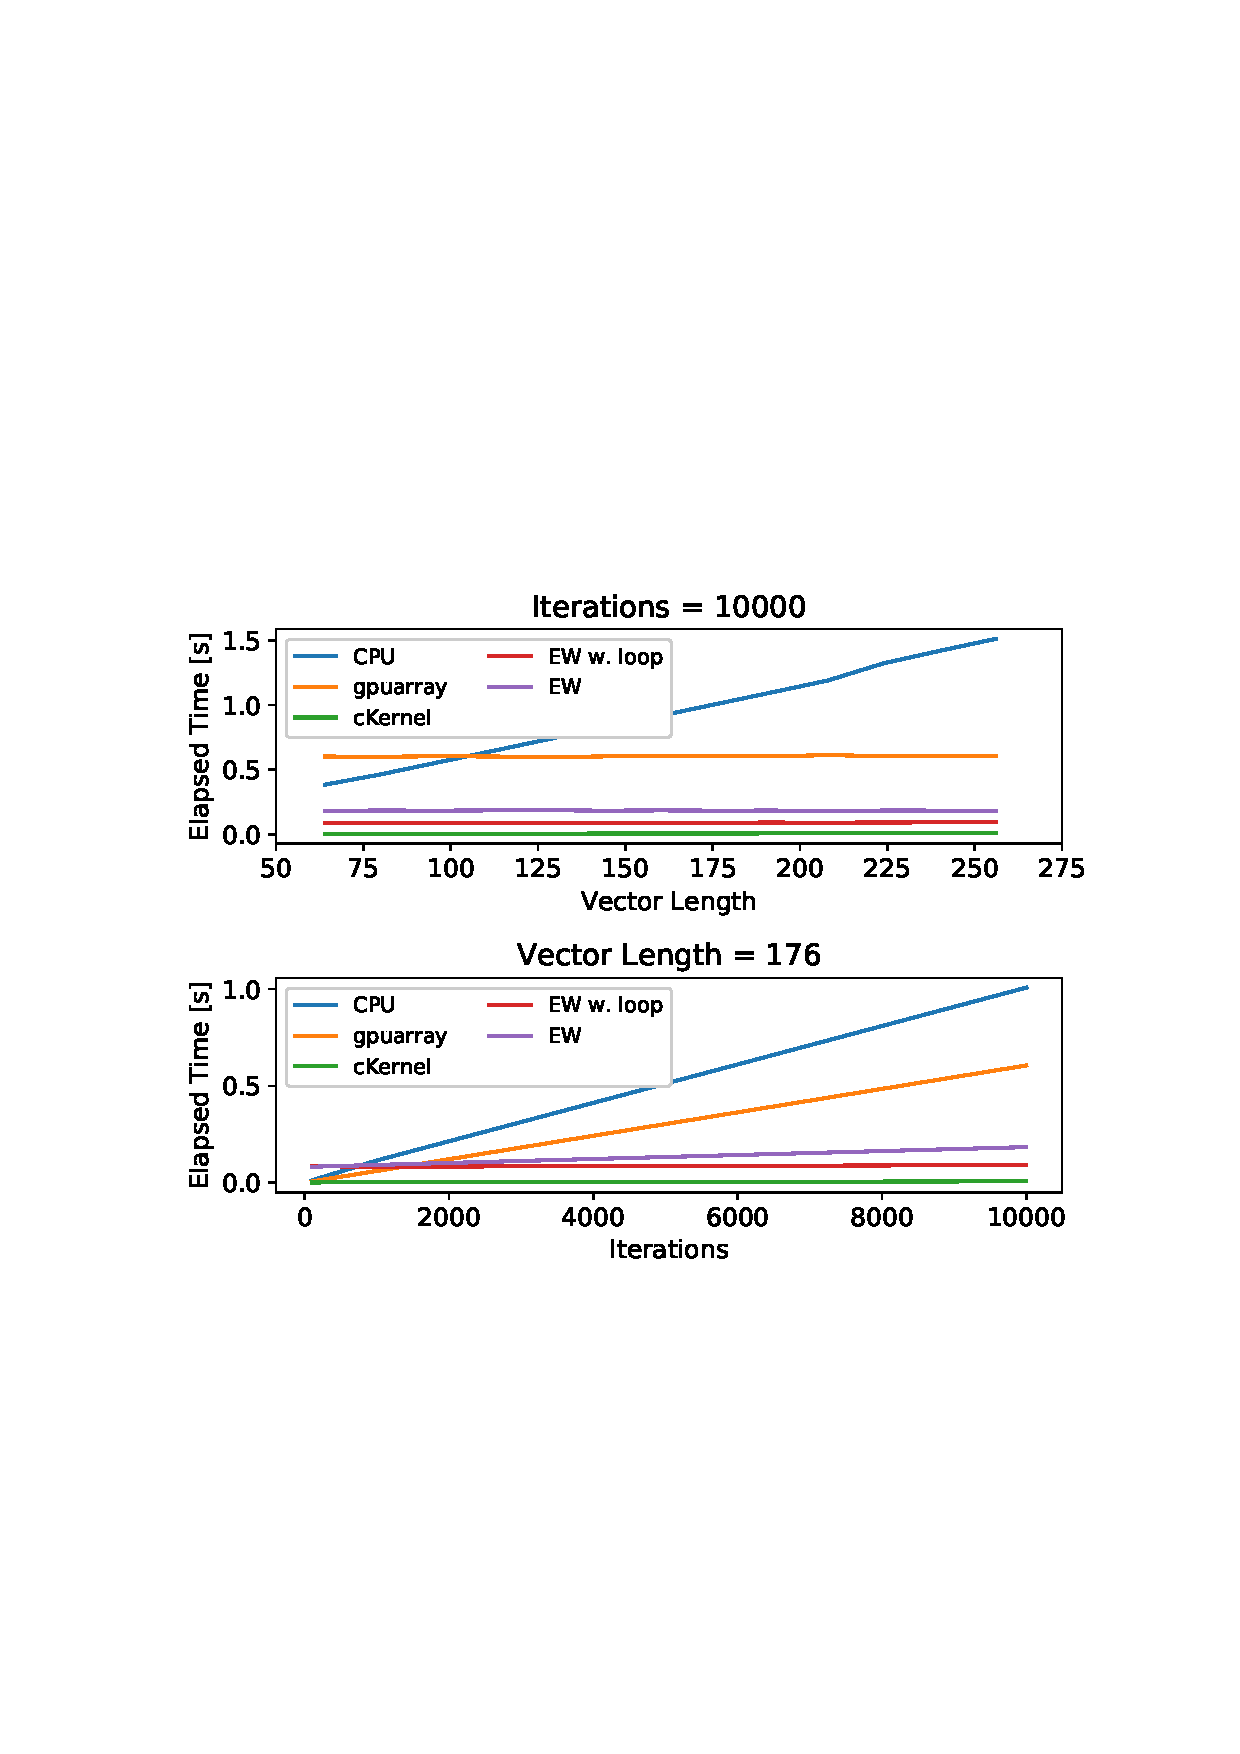
\includegraphics[width=0.7\textwidth]{benchmark002_outData_gaia_K80}
    \caption{Comparison of the run time of CPU, \texttt{gpuarray} method, \texttt{Elementwise} kernel (with internal \& external loop) and C kernel: Elapsed time of sine computation after 10.000 iterations and influence of number of iterations on the elapsed time}
    \label{benchmark_006}
\end{figure}

The graphs shown in Figure~\ref{benchmark_006} are obtained on Gaia. The C kernel is for all vector lengths and number of iterations the fastest. For a small number of iterations (less than around 1500) the \texttt{gpuarray} method performs better than the \texttt{Elementwise} kernels.

Looping on the GPU speeds up the computation. However, it is only feasible if each iteration operates on the same data, like computing 100 times the sine of the same matrix. If data changes and need to be updated, a copying operation prevents the usage of an internal loop on the GPU as used in the \texttt{Elementwise} kernel with internal loop and the C kernel.

\subsection{Matrix Multiplication on CPU vs. \texttt{gpuarray} vs. \texttt{Reduction} Kernel}

In this benchmark, single matrix multiplication of random, three dimensional matrices of order 64 to 512 in 16-increments is compared running on the CPU and on the GPU using \texttt{gpuarray} and a \texttt{Reduction} kernel. A comparison that included also a C kernel was attempted but returned incorrect values and was therefore discontinued. 

\begin{figure}[H]
    \centering
    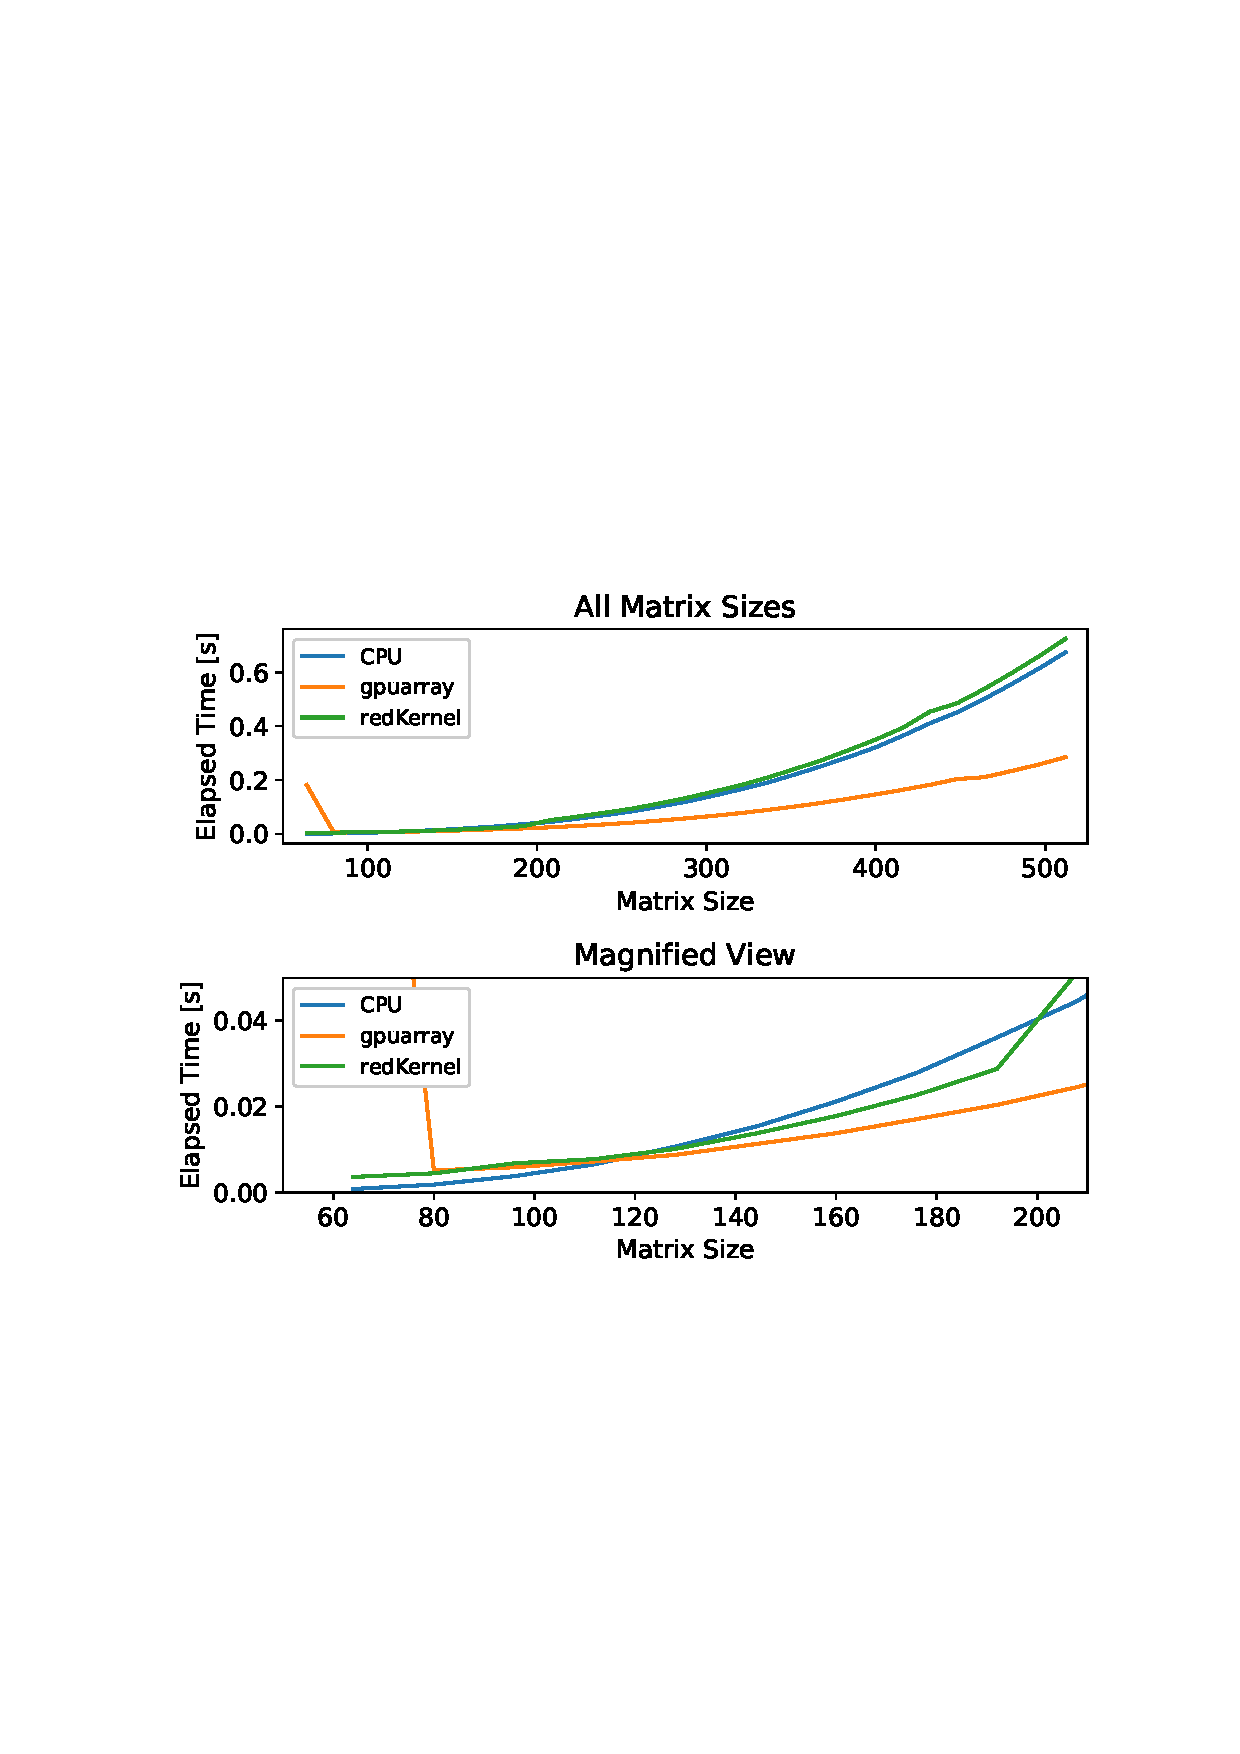
\includegraphics[width=0.7\textwidth]{benchmark003_outData_gaia_K80}
    \caption{Comparison of the run time of CPU, \texttt{gpuarray} method and \texttt{Reduction} kernel: Elapsed timeforf matrix multiplication of three-dimensional matrices of order \emph{Matrix Size}}
    \label{benchmark_007}
\end{figure}

The results shown in Figure~\ref{benchmark_007} are computed on Gaia. When called for the first time, the \texttt{gpuarray.dot()} method compiles a kernel, hence it takes longer time to execute in the first computation. For matrix orders bigger than 200, the \texttt{gpuarray.dot()} method performs the fastest. The \texttt{Reduction} kernel runs faster than the CPU for matrix orders between 120 and 200. This behavior can be observed on Tegner NVIDIA Tesla K420 as well, so is not only exclusive to Gaia nor to the NVIDIA Tesla K80. 

Finally, the \texttt{gpuarray} class offers the highest flexibility as much as decent speed-up when working with different matrix operations.

\section{import Final Implementation as Result}

The numpy arrays and scalars passed to the \texttt{bicgstab} function are converted to \texttt{gpuarray} and pushed to the GPU. A gpu version of the class \texttt{Unknown} is thereby used. The mathematical operations are carried out and saved on the GPU. The final array is fetched from the GPU and returned from the \texttt{bigcstab} function. Comparison operations in \texttt{bicgstab} are carried out on CPU since no comparison operator is defined in PyCUDA: they might be carried out on the GPU using \texttt{gpuarray.is\_positive()}, but this has not been tested yet.

The \texttt{mat\_vec\_bnd} subroutine operates on the GPU in the same way as on the CPU. The slicing is done on the GPU. In \texttt{vec\_vec}, the PyCUDA built-in \texttt{gpuarray.dot()} routine is used.

A boolean \emph{gpu} is set in the \texttt{bicgstab} function to enable the computation on the GPU. It is additionally passed as an input parameter to the subroutines which is per default false. 

As test case, the flow around four rectangular-shaped obstacles arranged in a labyrinth setting is computed for 200 time steps. The \texttt{bicgstab} function is called four times per times step: three times for solving each velocity component and a fourth time for the pressure. 

The maximal Courant-Friedrich-Lewy (CFL) number is compared to examine the accuracy of the computation on the GPU. It is important to note that 64 byte precision is needed to achieve sufficient results. The mid-plane velocity and pressure fields after 200 time steps are compared to ensure that differences lie in the order of numerical diffusion. Plots are shown in Appendix \ref{cfd_figs}.

The test case is run with different mesh sizes, displayed in Table~\ref{mesh_sizes}. The aspect ratio is specified in the table as the obstacles are scaled with the grid dimension. Equal aspect ratio ensures an equal physical problem.

\begin{table}[h]
    \centering
    \begin{tabular}{c|c|c}
     Mesh & Size & Aspect Ratio \\
     \hline
     1 & $ 64 \cdot  16 \cdot  16$ & 4:1  \\
     2 & $128 \cdot  16 \cdot  16$ & 8:1  \\
     3 & $128 \cdot  32 \cdot  32$ & 4:1  \\
     4 & $256 \cdot  32 \cdot  32$ & 8:1  \\
     5 & $256 \cdot  64 \cdot  64$ & 4:1  \\
     6 & $512 \cdot  64 \cdot  64$ & 8:1  \\
     7 & $512 \cdot 128 \cdot 128$ & 4:1
    \end{tabular}
    \caption{Mesh sizes used for computation and aspect ratio between main flow axis and the two orthogonal axes}
    \label{mesh_sizes}
\end{table}

Just like the benchmarks, the computations are run on the ULHPC Cluster Gaia on Intel Xeon E5-2680v3 CPUs and NVIDIA Tesla K80 GPUs when referred to Gaia. When referred to Tegner, the computations are carried out on KTH PDC Cluster Tegner on Intel E5-2690v3 Haswell CPUs and NVIDIA Tesla K80 GPUs. The code and simulation data can be found on github\footnote{\url{https://github.com/kjcramer/pyns/tree/HPC_SummerSchool/pycuda}}. The final simulation results are grouped in the corresponding folder (e.g. "gaia\_gpu/").

The computation times are averaged between 24 runs per mesh size on CPU Tegner and three runs per mesh size on CPU Gaia and the GPUs (both Tegner and Gaia). On CPU Tegner, one run per physical core of the node is performed simultaneously, whereas on CPU Gaia one simulation on one core per node is run.

In Figure~\ref{final_total_time} the total execution time of the full simulation is shown. Computation on the GPU is faster for mesh sizes larger than mesh 4 or 5. As the aspect ratio of the mesh is changing, the number of iterations in \texttt{bicgstab} might change and by that also the overall execution time.

In Figure~\ref{final_time_per_iteration} the average time per inner iteration in \texttt{bicgstab} for all calls of \texttt{bicgstab} is shown. Even though the slopes are slightly different, the critical mesh size stays the same. For larger mesh sizes, the time advantage of computing on the GPU increases significantly. On Gaia, while mesh 5 takes the same time to run on CPU and GPU, the GPU is already twice as fast for mesh 6. The speed-up of mesh 7 even increases to 5.6 meaning that a simulation takes a day instead of a working week.

On Tegner, when running a simulation on each core of the CPU node, already mesh 3 is 1.5 times faster on the GPU. For mesh 4 the speed-up is 4.4, for mesh 5 it is 6.9, for mesh 6 it is 6.6. Mesh 7 is nearly 12 times faster on the GPU.

\begin{figure}[H]
    \centering
    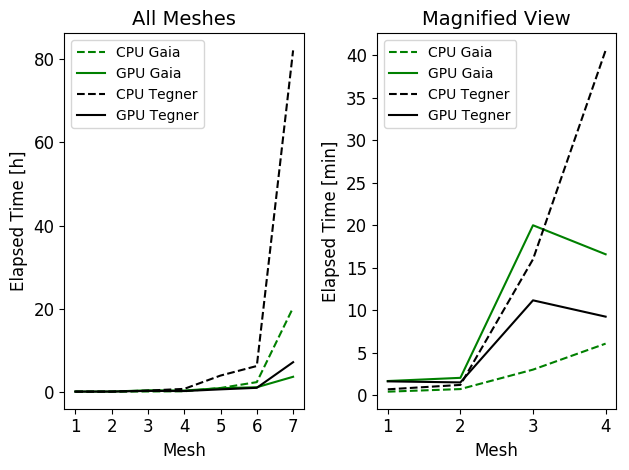
\includegraphics[width=0.71\textwidth]{Comparison_total_time.png}
    \caption{Comparison of the total execution time of 200 time steps for different mesh sizes computed on CPU and GPU}
    \label{final_total_time}
\end{figure}

\begin{figure}[H]
    \centering
    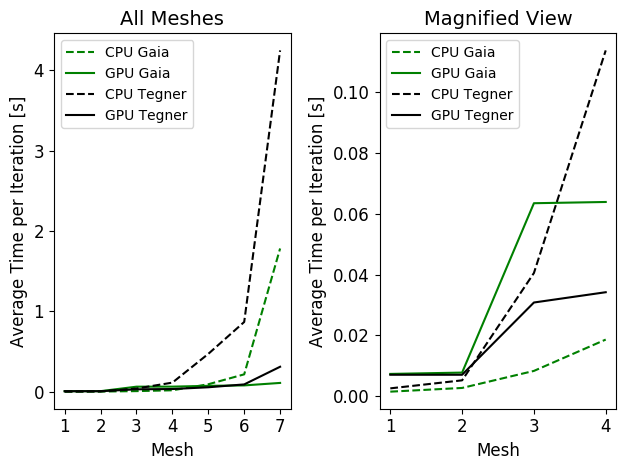
\includegraphics[width=0.71\textwidth]{Comparison_time_per_iteration.png}
    \caption{Comparison of the average time spent per iteration in \texttt{bicgstab} for different mesh sizes computed on CPU and GPU for 200 time steps}
    \label{final_time_per_iteration}
\end{figure}

\section{import Conclusion}

Looking at the results, the port of the numerical solver \texttt{bicgstab} can be considered successful: a simulation that would take a working week can now be performed in less than a working day.

PyCUDA is relatively easy to use, once its limits are understood and circumvented (e.g. multiplying a scalar with a matrix): with the \texttt{pycuda.gpuarray} library you don't need to be a programmer -- even mechanical engineers get somewhere without worrying about pointers. The documentation, scary at first, might be more understandable to trained computer scientists.

When working with CFD and numerical methods, 64 byte precision on the GPU is an absolute requirement. This might be a constraint for GPUs that lack hardware support for double precision numbers. Moreover, in case of a machine that has multiple users and only one GPU, there is no easy way to tell whether a process is already using the GPU or not. In an environment like a supercomputer, having to reserve a 24-cores node and using only its GPU is a potential waste of resources.

\section*{Acknowledgement}

We want to thank the people behind both PDC and ULHPC for being super-supportive and quick in replying to every question we encountered as engineers who dared to approach the field of computer science. 

\newpage

\begin{appendices}

\section{Setting up HPCs}

\subsection*{Running on PDC KTH Tegner}
\begin{enumerate}
\item \texttt{kinit --forwardable -l 7d manzari@NADA.KTH.SE}
\item \texttt{ssh USER@tegner.pdc.kth.se}
\item \texttt{salloc -t hh:mm:ss -N 1 -A summer-extra-2017 --gres=gpu:K420:1 [or K80:2]}
\item ssh directly to GPU node
\item \texttt{module load cuda anaconda}
\end{enumerate}

\subsection*{Running on ULHPC Gaia}
\begin{enumerate}
\item \texttt{ssh gaia}
\item \texttt{oarsub -t gpu -l nodes=1/core=2,walltime=hh:mm:ss ./myscript.sh}
\begin{itemize}
\item for specific node \texttt{-p "network\_address='gaia-182'"}
\item for specific GPU \texttt{-p "gputype='K80'"}
\item for batch job do header \texttt{\#!/bin/bash -l}
\end{itemize}
\end{enumerate}

\section{CFD Simulation Figures}
\label{cfd_figs}

\begin{figure}[H]
\centering
\begin{subfigure}[b]{\textwidth}
   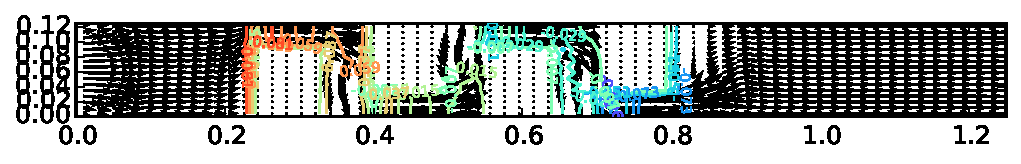
\includegraphics[width=1\linewidth]{fig1_t200_cpu.pdf}
   \caption{}
   \label{fig_cpu} 
\end{subfigure}

\begin{subfigure}[b]{\textwidth}
   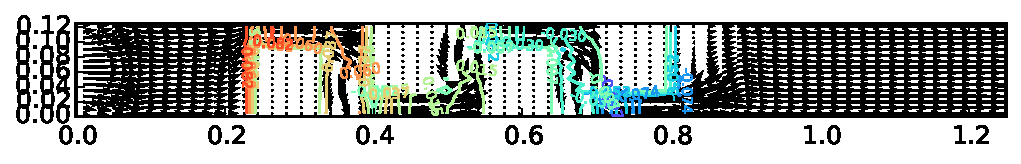
\includegraphics[width=1\linewidth]{fig1_t200_gpu.pdf}
   \caption{}
   \label{fig_gpu}
\end{subfigure}
\caption{Velocity (arrows) and pressure field of mesh 1 in the mid-z-plane after 200 time steps (a) run on CPU (b) run on GPU}
\end{figure}


\end{appendices}

\end{document}
